\documentclass[a4paper]{article}

%% Language and font encodings
\usepackage[english]{babel}
\usepackage[utf8x]{inputenc}
\usepackage[T1]{fontenc}
\usepackage{blindtext}
\usepackage{enumitem}
\usepackage{float}
\usepackage{commath}

%% Sets page size and margins
\usepackage[a4paper,top=3cm,bottom=2cm,left=3cm,right=3cm,marginparwidth=1.75cm]{geometry}

%% Useful packages
\usepackage{amsmath}
\usepackage{graphicx}
\usepackage[export]{adjustbox}
\usepackage[colorinlistoftodos]{todonotes}
\usepackage[colorlinks=true, allcolors=blue]{hyperref}

\setlength{\parskip}{0.5em}
\renewcommand{\baselinestretch}{1.2}

\title{State Obesity Intervention \\
A Difference-in-Difference Analysis}

\author{Eileen Xia \\ ECON20 Dartmouth College \\ Professor Dietrich Vollrath}

\date{\today}

\begin{document}
\maketitle

%%##########################################################################
\section{Research Design}
I chose to do a difference in difference analysis as it is the most appropriate analysis for the information provided. We have no information on how the people were chosen for the program. Thus, we cannot assume that assignment was random. The difference in difference method accounts for the fact that in the absence of random assignment, the treated and untreated groups can differ for many reasons. Using difference in difference allows us to adjust for pre-existing differences between the treated and untreated groups to better analyze the causal effect of treatment. We are able to do this through diff in diff by comparing the divergence in the trend of treated patients post-treatment from the trend of untreated, control patients. Diff in diff is also the best analysis to use because there are multiple periods. We have data from 2004 to 2012, where treatment occurs in 2007 and 2008. Using difference in difference, we can see the effect of the program during and after the treatment and as it changes over time.

%%##########################################################################
\section{Specification}

\subsection{Baseline Specification: 3 Periods}

The years range from 2004 to 2012, with treatment occurring in 2007 and 2008; there are multiple years pre, during, and post treatment. Because I am more interested in the variation in treatment effects during and after treatment rather than the variation in treatment effects year by year, I decided to create 3 periods. Hence, I set the variable \(period\) to 1 for years 2004 to 2006, 2 for years 2007 and 2008, and 3 for years 2009 to 2012. In a difference in difference analysis, observing the different periods during and post treatment account for the fact that conditions change for everyone over time, whether treated or not. Equations 1, Equation 2, and Equation 3 are the general interaction regressions for dependent variables \(heart\), \(er\), and \(employ\).

\begin{equation}
heart_{ij} = \delta_1 + \theta_1 Program_i + \sum_{j=2,3} \delta_j Period_j + \sum_{j=2,3} \theta_j Period_j * Program_i + u_{ij}
\end{equation}
\begin{equation}
er_{ij} = \delta_1 + \theta_1 Program_i + \sum_{j=2,3} \delta_j Period_j + \sum_{j=2,3} \theta_j Period_j * Program_i + u_{ij}
\end{equation}
\begin{equation}
employ_{ij} = \delta_1 + \theta_1 Program_i + \sum_{j=2,3} \delta_j Period_j + \sum_{j=2,3} \theta_j Period_j * Program_i + u_{ij}
\end{equation}

The value $\delta_1$ is a constant and is the vertical intercept. The coefficient $\theta_1$ indicates the initial difference in the level of outcome between the treated and untreated groups. Controlling for pre-existing differences allows us to make a better causal interpretation of the program on the outcome. The coefficient $\delta_j$ indicates the difference in outcome from the first period for untreated people; this accounts for the fact that everyone changes over time. The coefficient $\theta_j$ is what we are interested in; this value indicates the difference in difference in outcome from the first period for treated people. This value captures the causal effect of treatment by seeing how the trend for the treatment group changes from the common trend followed by the control group. For the period before the program starts, we expect the value of $\theta_j$ to be close to zero because treatment has not yet occurred. This is why we focus on periods 2 (during) and 3 (after); these values capture the causal effect of treatment. $u_{ij}$ is the error term.

The subscript $i$ associated with the dependent variables and error term indicates each individual/observation. The subscript $j$ on these same variables indicates the time period, 1 2 or 3. The subscript $i$ associated with the variable \(Program\) indicates whether individual $i$ received treatment or not. Because \(program\) is a dummy variable, $Program_i = 1$ indicates the individual got treatment and $Program_i = 0$ indicates the individual got no treatment. The subscript $j$ associated with \(Period\) and the corresponding coefficients indicate the period; recall that 1 indicates before treatment, 2 indicates during treatment, and 3 indicates after treatment. Thus, for y-variables $heart$, $er$, and $employ$, $y_{ij}$ and $u_{ij}$ are the outcome and error term for person $i$ in period $j$ respectively.

\subsection{Adding Controls}

In addition to the baseline specification, I want to control for variables that could effect my interpretation of the causal effect of treatment. As such, I control for age, education, and county. First, I control for age, then age and education, then all three of age, education, and county. I do this for each y-variable: heart, er, and employ. 

\begin{equation}
y_{ij} = \delta_1 + \theta_1 Program_i + \sum_{j=2,3} \delta_j Period_j + \sum_{j=2,3} \theta_j Period_j * Program_i + \beta_{1} age_i + u_{ij}
\end{equation}

\begin{equation}
y_{ij} = \delta_1 + \theta_1 Program_i + \sum_{j=2,3} \delta_j Period_j + \sum_{j=2,3} \theta_j Period_j * Program_i + \beta_{1} age_i + \beta_{2} educ_i + u_{ij}
\end{equation}

\begin{equation}
y_{ij} = \delta_1 + \theta_1 Program_i + \sum_{j=2,3} \delta_j Period_j + \sum_{j=2,3} \theta_j Period_j * Program_i + \beta_{1} age_i + \beta_{2} educ_i + \beta_{3} county_i + u_{ij}
\end{equation}
\\
The y-variable is in place for each of the dependent variables: heart, er, and employ. The subscripts are the same as in Equations 1, 2, and 3 which do not have control variables. The coefficient $\beta_{1}$ is the effect of age on the outcome. The coefficient $\beta_{2}$ is the effect of education on the outcome. The coefficient $\beta_{3}$ is the effect of county on outcome. The subscript $i$ on age, educ, and county indicate the specific age, education, and county of individual $i$.

The age, education, and county variables are observables that could potentially be related to the outcome, which could present bias in our estimated coefficients. Thus, I add these variations to the baseline specification because I want to see how doing so effects my estimate for $\theta_j$, the coefficient that captures the causal effect of treatment. If there is a significant change in my estimate for $\theta_j$, this means the control variables used have a significant impact on the outcome, and that the estimate for $\theta_j$ from the baseline specification is biased. On the other hand, if there is not a significant change in $\theta_j$ from the baseline specification, I am more convinced that the causal effect portrayed in the estimate of $\theta_j$ is closer to the actual effect.

\subsection{Year by Year Specification}

I am also curious to see how the treatment effect varies by year and whether these variations provide information not seen in the regression specified by Equations 6. As such, I will run a regression interacting treatment with each year, as specified in the following equation:

\begin{equation}
y_{it} = \delta_{2004} + \theta_{2004} Program_i + \sum_{t=2005}^{2012} \delta_t Year_t + \sum_{t=2005}^{2012} \theta_t Year_t * Program_i + \beta_{1} age_i + \beta_{2} educ_i + \beta_{3} county_i + u_{it}
\end{equation}

We run this regression for the $y$ variables $heart$, $er$, and $employ$. The coefficient $\delta_{2004}$ is a constant and represents the vertical intercept. The coefficient $\theta_{2004}$ is the initial difference in the level of outcome between the treatment and control groups in 2004. The coefficient $\delta_t$ is the difference in outcome from the first year, 2004, for untreated individuals. We are interested in the coefficient $\theta_t$ because this value is the difference in difference in outcome in year $t$ from the first year, 2004, for treated individuals. For years 2005 and 2006, we expect for $\theta_t$ to be zero because treatment has not started. Thus, we are interested in $\theta_t$ for years $t$ = 2007 to 2012 because they capture the causal effect of treatment. Same as before, $\beta_{1}$, $\beta_{2}$, and $\beta_{3}$ capture the effects of age, education, and county on the outcome, respectively. Program is the dummy for treatment and Year denotes the year.

The subscript $i$ on the dependent variable $y$ and error term $u$ denotes each person observed. Again, the subscript $i$ on Program indicates whether person $i$ received treatment (program = 1) or not (program = 0). The subscript $t$ on $y$, $\delta$, $\theta$, and $Year$ is the year, from 2005 to 2012. The subscript $i$ on control variables age, educ, and county are the corresponding ages, education levels, and county of residence for person $i$.

The year by year regression paints a more detailed picture of the effect of treatment because it looks at the difference in difference in outcome each year rather than for multiple years grouped by period.

\subsection{Calculating Standard Errors}
The homoskedasticity assumption is that the error variance is a constant for any value of the independent variable. In other words, $Var(u|x_1, …, x_k) = \sigma^{2}$. If the variance changes with any explanatory variable, this assumption is violated; the error term exhibits heteroskedasticity and variance, $Var(u_i) = \sigma_{i}^{2}$, varies by individual

It is unknown if the models I have specified above exhibit homoskedasticity. I will not assume they exhibit homoskedasticity because if heteroskedasticity is at all present, statistical inference procedures are invalidated. Although heteroskedasticity presents no bias/inconsistencies in our coefficient estimates or usual and adjusted R-squared, the estimators of variances are biased. Because the standard errors are directly derived from the estimated variances, they change and are invalid for constructing t-stats and confidence intervals, preventing hypothesis testing. 

Because the skedasticity of the specified models are unknown, I will calculate standard errors so that they are valid for statistical inference in the case that there exists heteroskedasticity of unknown form. To do so, I use robust standard errors; robust procedures are valid whether error variances are constant or not. 

The robust procedure introduces adjustments in calculating the estimator of variance, and thus standard error. The robust standard error for a coefficient is the square root of the estimated variance of the coefficient. The valid estimator of variance is calculated as the covariance of each squared $x_i$ and squared residuals $\hat{u_i}$. The farther $x_i$ is from the mean value of x, the larger the squared deviations in x; the squared deviation is greatest at the ends of the range near the minimum and maximum values of x. Thus, if the residuals are large at the ends, the estimator of variance is large and our robust standard error is larger than a normal standard error. Likewise, if the residuals are large near the mean of x, the robust standard error is smaller than the normal standard error.

Robust standard errors are valid more often than usual standard errors and should always be used when it is unknown whether the homoskedasticity assumption holds, especially for very large sample sizes like the data we use here.


%%##########################################################################
\section{Data}
My first step was to summarize all of the initial data. In Table 1 we see the summary of the untouched variables. We see from $id$ that we observe 6708 individuals. There are 60,372 total observations because we observe each person for 9 years, 2004 to 2012. $program$ is a dummy variable indicating whether a person received treatment or not. We have information about each person's level of education $educ$, $age$, and weeks of employment per year $employ$.

\begin{table}[H]
\caption{initial data}
\centering
\begin{tabular}{|r|r|r|r|}
{
\def\sym#1{\ifmmode^{#1}\else\(^{#1}\)\fi}
\begin{tabular}{l*{1}{cccccc}}
\hline\hline
            &       count&        mean&         Var&          sd&         min&         max\\
\hline
id          &       60372&      3354.5&     3749834&    1936.449&           1&        6708\\
year        &       60372&        2008&    6.666777&     2.58201&        2004&        2012\\
program     &       60372&    .3252832&    .2194777&    .4684845&           0&           1\\
educ        &       59134&    13.99373&    2.003901&    1.415592&          12&          16\\
county      &       60372&    25.31246&    209.4902&    14.47378&           1&          50\\
age         &       59177&    31.55875&    15.01937&    3.875483&          23&          40\\
employ      &       59775&    26.30642&    365.6227&    19.12126&           0&          50\\
heart       &       59769&    157.1371&     1459168&     1207.96&        4.25&        9999\\
er          &       60372&    .9163851&    .6597193&     .812231&           0&           2\\
\hline
\(N\)       &       60372&            &            &            &            &            \\
\hline\hline
\end{tabular}
}

\end{tabular}
\end{table}

An important observation is that there are a total of 60,372 observations; variables that do not have this number of observations are missing data. The variables missing data are thus \(educ\), \(age\), \(employ\), and \(heart\). 

With this information, we can make modifications to the data. First, I replaced the missing data in the education and age variables because there is enough information to do so. We should avoid missing data if we can. For a particular individual, the number of years of education is a constant. I can assume that no individual in the data set is currently in school because no individual has a changing education value. Thus, if there is a missing value for education, I look at the education data for the individual from a year in which this data isn’t missing and replace the missing cell with the correct value. I created a new variable \(educfull\) to hold the data for education with no missing values. Similarly, a person’s age increments by one each year. Thus, we take age data for an individual from a year that isn’t missing age information and calculate the corresponding age of the individual for the missing year. The variable \(agefull\) holds the data for age with zero missing values. 

Unlike \(educ\) and \(age\) values, missing data for \(employ\) and \(heart\) cannot be filled in. However, in Table 1 we see there is a surprising value for the max of heart, 9999. Given that the mean is around 157, this value for heart seems extreme and definitely is not the actual value of a person's heart health; oddly specific numbers like 9999 are likely mismeasured, so I assume this value is probably used to code for missing. As such, I replace all values of heart equal to 9999 as missing. 

For all other variables, the min and max values do not indicate the existence of any extreme outliers. Table 2 shows the summary of the final data that I will use in my analysis.

\begin{table}[H]
\caption{final data}
\centering
\begin{tabular}{|r|r|r|r|}
{
\def\sym#1{\ifmmode^{#1}\else\(^{#1}\)\fi}
\begin{tabular}{l*{1}{cccccc}}
\hline\hline
            &       count&        mean&         Var&          sd&         min&         max\\
\hline
educfull    &       60372&    13.99299&    2.003711&    1.415525&          12&          16\\
agefull     &       60372&    31.56321&    15.03039&    3.876905&          23&          40\\
employ      &       59775&    26.30642&    365.6227&    19.12126&           0&          50\\
heart       &       58882&    8.878993&    8.481532&    2.912307&        4.25&    21.14268\\
er          &       60372&    .9163851&    .6597193&     .812231&           0&           2\\
\hline
\(N\)       &       60372&            &            &            &            &            \\
\hline\hline
\end{tabular}
}

\end{tabular}
\end{table}

%%##########################################################################

\section{Results}

\subsection{Program Effect on Heart Health}
Table 3 shows the results of running the regressions specified by Equation 1, Equation 4, Equation 5, and Equation 6 respectively, where $y$ is heart. The first column is the baseline specification where no controls are used. Column 2 controls for age, Column 3 controls for age and education, and Column 4 controls for age, education, and county. The estimated coefficient on "Program dummy" is $\hat{\theta_{1}}$, the estimated coefficient on "During treatment" is $\hat{\delta_{2}}$, the estimated coefficient on "After treatment" is $\hat{\delta_{3}}$, the estimated coefficient on "Program dummy*During treat" is $\hat{\theta_{2}}$, and the estimated coefficient on "Program dummy*After treat" is $\hat{\theta_{3}}$. 

\begin{table}[H]
\centering
\begin{table}[htbp]\centering
\def\sym#1{\ifmmode^{#1}\else\(^{#1}\)\fi}
\caption{Dependent variable: Heart}
\begin{tabular}{l*{4}{c}}
\hline\hline
            &\multicolumn{1}{c}{(1)}&\multicolumn{1}{c}{(2)}&\multicolumn{1}{c}{(3)}&\multicolumn{1}{c}{(4)}\\
            &\multicolumn{1}{c}{heart}&\multicolumn{1}{c}{heart}&\multicolumn{1}{c}{heart}&\multicolumn{1}{c}{heart}\\
\hline
Program dummy&     -0.9272\sym{***}&     -0.9257\sym{***}&     -0.9359\sym{***}&     -0.9294\sym{***}\\
            &    (0.0434)         &    (0.0434)         &    (0.0423)         &    (0.0424)         \\
[1em]
During treatment&     -0.0792\sym{**} &     -0.0586         &     -0.0726\sym{*}  &     -0.0734\sym{*}  \\
            &    (0.0339)         &    (0.0405)         &    (0.0394)         &    (0.0394)         \\
[1em]
After treatment&     -0.0545         &     -0.0425         &     -0.0463         &     -0.0465         \\
            &    (0.0403)         &    (0.0425)         &    (0.0411)         &    (0.0412)         \\
[1em]
Program dummy*During treat&      0.3367\sym{***}&      0.3348\sym{***}&      0.3373\sym{***}&      0.3374\sym{***}\\
            &    (0.0575)         &    (0.0575)         &    (0.0561)         &    (0.0561)         \\
[1em]
Program dummy*After treat&      0.8148\sym{***}&      0.8132\sym{***}&      0.8152\sym{***}&      0.8154\sym{***}\\
            &    (0.0682)         &    (0.0682)         &    (0.0662)         &    (0.0662)         \\
[1em]
Controls for age &          No         &         Yes         &         Yes         &         Yes         \\
[1em]
Controls for education &          No         &          No         &         Yes         &         Yes         \\
[1em]
Controls for county &          No         &          No         &          No         &         Yes         \\
\hline
\(N\)       &       58882         &       58882         &       58882         &       58882         \\
\(R^{2}\)   &       0.012         &       0.013         &       0.068         &       0.068         \\
adj. \(R^{2}\)&       0.012         &       0.012         &       0.067         &       0.067         \\
p-value 1.program=0&      0.0000         &      0.0000         &      0.0000         &      0.0000         \\
p-value 2.period=0&      0.0195         &      0.1479         &      0.0652         &      0.0625         \\
p-value 3.period=0&      0.1766         &      0.3169         &      0.2610         &      0.2588         \\
p-value 1.program#2.period=0&      0.0000         &      0.0000         &      0.0000         &      0.0000         \\
p-value 1.program#2.period=0&      0.0000         &      0.0000         &      0.0000         &      0.0000         \\
\hline\hline
\multicolumn{5}{l}{\footnotesize Standard errors in parentheses}\\
\multicolumn{5}{l}{\footnotesize \sym{*} \(p<0.10\), \sym{**} \(p<0.05\), \sym{***} \(p<0.01\)}\\
\end{tabular}
\end{table}

\end{table}

First I look at the estimated coefficients for the baseline specification. The estimate for "Program dummy" tells us the pre-existing difference in heart health between the treated and untreated groups; treated individuals had worse heart health by 0.9272 before treatment began. The "During treatment" result shows how untreated individuals' heart health changed over time. From the before period, 2004-2006, to the during period, 2007-2008, untreated individuals' heart health dropped by 0.0792. Similarly, the "After treatment" result shows that from the before period to the after period, 2009-2012, untreated individuals' heart health had dropped by 0.0545. The interaction effects are the causal effect of treatment. The estimate for "Program dummy*During treat* tells us treated individuals' heart health improved by 0.3367 relative to the untreated individuals' drop of 0.0792 during this time; in other words their heart health went up by 0.2575. If we take this estimated coefficient as the causal effect of treatment, this means that treatment improved heart health by 0.3367 from before treatment to the time treatment was occurring. Similarly, the estimate for "Program dummy*After treat" tells us treated individuals' heart health after treatment ended had overall improved 0.8148 relative to the untreated individuals' drop of 0.0545; their heart health improved by 0.7603. Again, if we take this estimated coefficient to be the causal effect of treatment, this means that treatment improved heart health by 0.8148 from before treatment to after treatment ended.

We cannot be sure that the estimated coefficients $\hat{\theta_{2}}$ and $\hat{\theta_{3}}$ are the causal effects of treatment. For further insight into the effect of treatment, we must compare the values of the estimated coefficients to the estimated coefficients when we control for certain variables. For each of the specifications with added controls, we see minimal changes in "Program dummy", "During treatment", and "After treatment" estimates. More importantly, we see very little change in "Program dummy*During treat" and "Program dummy*After treat" estimates. When we control for age, we see $\hat{\theta_{2}}$ barely changes and is still around 0.33. $\hat{\theta_{3}}$ also barely changes and is still around 0.81. The same is to be said when we control for both age and education, and also for when we control for age, education, and county together. Although this doesn't prove causality of treatment, this result does indicate that the control variables have very little effect on outcome.

When I conduct an F test on the null hypothesis $H_{0}: \beta_{1} = 0, \beta_{2} = 0, \beta_{3} = 0$, I reject the null at the 1$\%$ level. This indicates that at least one of $\beta_{1}$, $\beta_{2}$, or $\beta_{3}$ is different from zero. Hence, the control variables age, educ, and county are jointly statistically significant at the 1$\%$ level. We are interested in the estimated coefficients for the interaction terms; as such, I will use the result of the regression in Table 3's column 4 for the following analyses because the effects of age, education, and county are eliminated.

For all regressions, the p-value for the estimated coefficient $\hat{\theta_2}$ is sufficiently small; to 4 decimal points, the p-value is 0.0000. This means we reject the null that $\theta_2 = 0$ at the 1$\%$ level; $\hat{\theta_2}$ is statistically significant at the 1$\%$ level. The p-value for the coefficient estimate $\hat{\theta_3}$ is the same, 0.0000. Likewise, $\hat{\theta_2}$ is statistically significant at the 1$\%$ level and we reject the null that $\theta_3 = 0$.

However, statistical significance is not necessarily indicative of economic significance. We are using a large sample size of over 6,000 people; parameters can be estimated very precisely so the standard errors are small relative to the estimates, resulting in statistical significance. Therefore we look at the magnitude of $\hat{\theta_2}$ and $\hat{\theta_3}$ to truly determine economic significance.

There is no explicit interpretation for a person's heart value, but we see from Table 2 that heart ranges from 4.25 to 21.14. So for a value that has a range of around 17, an improvement in heart health by 0.3374 from before treatment to the time treatment was occurring seems economically insignificant. The improvement in heart health of 0.8154 from before treatment to after treatment is more than double this, however, and could be interpreted as minimally economically significant. An improvement of 0.8 in a range of 17 corresponds to less than 5$\%$ improvement. When compared to the mean heart value of around 8, this corresponds to around a 10$\%$ improvement.

For a variable like heart that is arbitrarily defined, deeming a finding economically significant is highly interpretive. In trying to analyze whether the result is economically significant, there are many things to think about. Consider the fact that all individuals observed were targeted for the program because they had risk factors associated with obesity; obesity causes many heart problems, so the observed population most likely has lower heart values than the general healthy population. Such little improvement in what is probably already a low heart value makes me inclined to say the treatment is economically insignificant, especially because the during and after treatment periods span years. However, we don't know how heart value is calculated and assigned. Although obesity causes heart problems that can go away by becoming healthy, obesity can leave long-lasting and even permanent effects on heart health, particularly if you are predisposed to poor heart health. It might not even be possible to see a heart value increase more than a couple of integers. I conclude that the treatment is economically significant, albeit minimally. I am further convinced the findings are economically significant because they are statistically significant at 1$\%$; using a smaller significance means that economic and statistical significance are more likely to coincide.


\subsection{Program Effect on Trips to the ER}

Table 4 shows the results of running the regressions specified by Equation 2, Equation 4, Equation 5, and Equation 6 respectively, where $y$ is er. The table follows the same format as Table 3 above. 

\begin{table}[H]
\centering
\begin{table}[htbp]\centering
\def\sym#1{\ifmmode^{#1}\else\(^{#1}\)\fi}
\caption{Dependent variable: Er}
\begin{tabular}{l*{4}{c}}
\hline\hline
            &\multicolumn{1}{c}{(1)}&\multicolumn{1}{c}{(2)}&\multicolumn{1}{c}{(3)}&\multicolumn{1}{c}{(4)}\\
            &\multicolumn{1}{c}{er}&\multicolumn{1}{c}{er}&\multicolumn{1}{c}{er}&\multicolumn{1}{c}{er}\\
\hline
Program dummy&     -0.2585\sym{***}&     -0.2589\sym{***}&     -0.2588\sym{***}&     -0.2588\sym{***}\\
            &    (0.0118)         &    (0.0118)         &    (0.0118)         &    (0.0119)         \\
[1em]
During treatment&      0.0004         &      0.0000         &     -0.0001         &     -0.0002         \\
            &    (0.0093)         &    (0.0111)         &    (0.0111)         &    (0.0111)         \\
[1em]
After treatment&     -0.0043         &     -0.0055         &     -0.0055         &     -0.0055         \\
            &    (0.0111)         &    (0.0117)         &    (0.0117)         &    (0.0117)         \\
[1em]
Program dummy*During treat&     -0.0040         &     -0.0036         &     -0.0036         &     -0.0036         \\
            &    (0.0157)         &    (0.0157)         &    (0.0157)         &    (0.0157)         \\
[1em]
Program dummy*After treat&      0.0020         &      0.0023         &      0.0023         &      0.0023         \\
            &    (0.0187)         &    (0.0187)         &    (0.0187)         &    (0.0187)         \\
[1em]
Controls for age &          No         &         Yes         &         Yes         &         Yes         \\
[1em]
Controls for education &          No         &          No         &         Yes         &         Yes         \\
[1em]
Controls for county &          No         &          No         &          No         &         Yes         \\
\hline
\(N\)       &       60372         &       60372         &       60372         &       60372         \\
\(R^{2}\)   &       0.022         &       0.023         &       0.023         &       0.024         \\
adj. \(R^{2}\)&       0.022         &       0.023         &       0.022         &       0.023         \\
p-value 1.program=0&      0.0000         &      0.0000         &      0.0000         &      0.0000         \\
p-value 2.period=0&      0.9651         &      0.9970         &      0.9944         &      0.9887         \\
p-value 3.period=0&      0.6952         &      0.6385         &      0.6378         &      0.6371         \\
p-value 1.program#2.period=0&      0.7968         &      0.8179         &      0.8178         &      0.8177         \\
p-value 1.program#2.period=0&      0.9160         &      0.9004         &      0.9004         &      0.9004         \\
\hline\hline
\multicolumn{5}{l}{\footnotesize Standard errors in parentheses}\\
\multicolumn{5}{l}{\footnotesize \sym{*} \(p<0.10\), \sym{**} \(p<0.05\), \sym{***} \(p<0.01\)}\\
\end{tabular}
\end{table}

\end{table}

Again, I start by looking at the estimated coefficients for the baseline specification in column 1. The estimate for “Program dummy” says the pre-existing difference is -0.2585; the people in the treated group had 0.2585 fewer trips to the ER than in the untreated group. The estimate for “During treatment” is 0.0004; this means that from the before period to the treated period, untreated individuals’ trips to the ER increased by 0.0004. The estimate for “After treatment” is -0.0043; compared to the before period, the people in the untreated group reduced their trips to the ER by 0.0043 in the after period. The estimate for “Program dummy*During treat” is the first estimate of interest; the estimate of -0.0040 indicates that individuals in the treated group reduced their trips to the ER by 0.0040 relative to the untreated individuals’ increase of 0.0004; in other words they reduced trips to the ER by 0.0036. Interpreting this estimate as the causal effect of treatment, this means treatment reduced trips to the ER by 0.0040 from before treatment to during treatment. The estimate for "Program dummy*After treat" is the second estimate of interest; the estimate of 0.0020 indicates that individuals in the treated group increased their trips to the ER by 0.0020 relative to the untreated individuals’ reduction of 0.0043. In other words they reduced trips to the ER by 0.0023. Interpreting this estimate as the causal effect of treatment, this means treatment actually increased trips to the ER by 0.0020 from before treatment to after treatment. 

It is interesting how the signs on the coefficient estimates for the interaction terms change from negative to positive; if the estimates are statistically significant, this could mean that the effect of treatment on ER trips doesn’t last once treatment ends. However, as I explain below, the estimate is both statistically and economically insignificant and thus the sign change doesn’t explain much.

We look to the regressions with control variables to see how the estimated coefficients $\hat{\theta_{2}}$ and $\hat{\theta_{3}}$ change. There are minimal changes in the estimate for "Program dummy"; the largest change is 0.0004 from the baseline estimate -0.2585. There are also minimal changes in "During treatment"; the largest change is 0.0006. The estimate for “After treatment” changes from -0.0043 to -0.0055 for all of the following regressions; again, this change is minimal. We are most interested to see how the estimates for "Program dummy*During treat" and "Program dummy*After treat" change. The “Program dummy*During treat” estimate changed minimally by 0.0004 from -0.0040 to -0.0036 when we control for age; the estimate is still -0.0036 when we add controls for education and then county. The “Program dummy*After treat” estimate also changed minimally by 0.0003 from 0.0020 to 0.0023 when we control for age; the estimate remains 0.0023 when we add control for education and county. Adding controls has no significant impact on the estimates.

To see the joint statistical significance of the three control variables, I conduct an F test on the null hypothesis $H_{0}: \beta_{1} = 0, \beta_{2} = 0, \beta_{3} = 0$ and find that age, education, and county are jointly statistically significant at the 10.49 $\%$ level. We barely fail to reject the null at the 10$\%$ level but reject the null at the 20$\%$ level; the control variables age, educ, and county are jointly statistically significant at the 20$\%$ level. I will use the result of the regression in Table *'s column 4 for the following analyses because we eliminate the effects of age, education, and county.

For all regressions, the p-value for the estimated coefficient on "Program dummy*During treat" is 0.79 or greater; this is quite large and we clearly fail to reject the null that $\theta_2 = 0$ at the 10$\%$ level; $\hat{\theta_2}$ is statistically insignificant at the 10$\%$ level. For all regression, the p-value for the estimated coefficient on  "Program dummy*After treat" is 0.90 or greater; again we fail to reject the null that $\theta_3 = 0$ at the 10$\%$ level; $\hat{\theta_3}$ is statistically insignificant at the 10$\%$ level. 

It is possible for a finding to be statistically insignificant but economically significant; this can happen when the sample size is small and there is little statistical power. However, in this particular case, the sample size is objectively large, with more than 6,000 people. This makes me very confident that the effect of treatment on visits to the ER is economically insignificant. First, the estimated coefficients on the interaction terms are very small. During treatment, the effect on ER visits is -0.0036. Although the number of trips to the ER is small, ranging from 0 to 2 as seen in Table 2, a drop of 0.0036 is still only a tiny 0.18$\%$ movement in the range for number of ER visits. The effect on ER visits is even smaller after treatment, with an increase in trips to the ER by 0.0023. Regardless, the findings are economically insignificant.

\subsection{Program Effect on Weeks of Employment}

Table 5 shows the results of running the regressions specified by Equation 3, Equation 4, Equation 5, and Equation 6 respectively, where $y$ is employ. The table follows the same format as Table 3 and Table 4 above. 

\begin{table}[H]
\centering
\begin{table}[htbp]\centering
\def\sym#1{\ifmmode^{#1}\else\(^{#1}\)\fi}
\caption{Dependent variable: Employ}
\begin{tabular}{l*{4}{c}}
\hline\hline
            &\multicolumn{1}{c}{(1)}&\multicolumn{1}{c}{(2)}&\multicolumn{1}{c}{(3)}&\multicolumn{1}{c}{(4)}\\
            &\multicolumn{1}{c}{employ}&\multicolumn{1}{c}{employ}&\multicolumn{1}{c}{employ}&\multicolumn{1}{c}{employ}\\
\hline
Program dummy&      1.1784\sym{***}&      1.1895\sym{***}&      1.1817\sym{***}&      1.2195\sym{***}\\
            &    (0.2888)         &    (0.2887)         &    (0.2887)         &    (0.2893)         \\
[1em]
During treatment&     -0.4965\sym{**} &     -0.3918         &     -0.4097         &     -0.4227         \\
            &    (0.2191)         &    (0.2632)         &    (0.2631)         &    (0.2633)         \\
[1em]
After treatment&     -0.3106         &     -0.2280         &     -0.2357         &     -0.2407         \\
            &    (0.2610)         &    (0.2758)         &    (0.2756)         &    (0.2756)         \\
[1em]
Program dummy*During treat&      0.1627         &      0.1492         &      0.1520         &      0.1531         \\
            &    (0.3827)         &    (0.3826)         &    (0.3825)         &    (0.3826)         \\
[1em]
Program dummy*After treat&      1.0244\sym{**} &      1.0141\sym{**} &      1.0178\sym{**} &      1.0181\sym{**} \\
            &    (0.4509)         &    (0.4509)         &    (0.4507)         &    (0.4508)         \\
[1em]
Controls for age &          No         &         Yes         &         Yes         &         Yes         \\
[1em]
Controls for education &          No         &          No         &         Yes         &         Yes         \\
[1em]
Controls for county &          No         &          No         &          No         &         Yes         \\
\hline
\(N\)       &       59775         &       59775         &       59775         &       59775         \\
\(R^{2}\)   &       0.002         &       0.002         &       0.003         &       0.004         \\
adj. \(R^{2}\)&       0.001         &       0.002         &       0.003         &       0.003         \\
p-value 1.program=0&      0.0000         &      0.0000         &      0.0000         &      0.0000         \\
p-value 2.period=0&      0.0235         &      0.1366         &      0.1194         &      0.1084         \\
p-value 3.period=0&      0.2341         &      0.4085         &      0.3924         &      0.3825         \\
p-value 1.program#2.period=0&      0.6707         &      0.6967         &      0.6911         &      0.6890         \\
p-value 1.program#2.period=0&      0.0231         &      0.0245         &      0.0239         &      0.0239         \\
\hline\hline
\multicolumn{5}{l}{\footnotesize Standard errors in parentheses}\\
\multicolumn{5}{l}{\footnotesize \sym{*} \(p<0.10\), \sym{**} \(p<0.05\), \sym{***} \(p<0.01\)}\\
\end{tabular}
\end{table}

\end{table}

As before, I start by looking at the estimated coefficients for the baseline specification in column 1. The estimate for “Program dummy” says the pre-existing difference is 1.1784; the people in the treated group were employed for 1.1784 more weeks than in the untreated group. The estimate for “During treatment” is -0.4965; this means that untreated individuals were employed for 0.4965 fewer weeks in the during period than the before period. The estimate for “After treatment” is -0.3106; compared to the before period, the people in the untreated group worked 0.3106 fewer weeks than in the after period. The estimate for “Program dummy*During treat” is the first estimate of interest; the estimate of 0.1627 indicates that individuals in the treated group were employed for 0.1627 more weeks relative to the untreated individuals’ 0.4965 decrease in weeks of employment. In other words, treated individuals were employed 0.3338 fewer weeks during the treatment period as compared to before the treatment period. Interpreting this estimate as the causal effect of treatment, this means treatment increased weeks of employment by 0.1627 from before treatment to during treatment. The estimate for "Program dummy*After treat" is the second estimate of interest; the estimate of 1.0244 indicates that individuals in the treated group were employed for 1.0244 weeks more than the untreated individuals’ drop of 0.3106. In other words they were employed for 0.7138 more weeks. Interpreting this estimate as the causal effect of treatment, this means treatment actually increased weeks of employment by 1.0244 from before treatment to after treatment. 

We want to see how the estimated coefficients $\hat{\theta_{2}}$ and $\hat{\theta_{3}}$ change when we add control variables. Adding controls increases the coefficient estimate on “Program dummy”; with all three controls the estimate increases to 1.2195, a change of 0.0411. Adding controls reduces the magnitude of the coefficient estimate on “During treatment”; with all three controls the estimate becomes -0.4227, a change of 0.0738. The magnitude of the coefficient estimate on “After treatment” decreases with controls; the estimate with all three controls is -0.2407, a 0.0699 change. More importantly, adding controls had less effect on the coefficient estimates on "Program dummy*During treat" and "Program dummy*After treat" but made them decrease nonetheless. The estimate for  "Program dummy*During treat" with all three controls became 0.1531, a 0.0096 change. The estimate for “Program dummy*After treat” with all three controls became 1.0181, a 0.0063 change. Adding controls has no significant effect on the estimates.

I determine the joint statistical significance of the three control variables with an F test on the null hypothesis $H_{0}: \beta_{1} = 0, \beta_{2} = 0, \beta_{3} = 0$. I reject the null at the 1$\%$ level; the control variables age, educ, and county are jointly statistically significant at the 1$\%$ level. This indicates that at least one of $\beta_{1}$, $\beta_{2}$, or $\beta_{3}$ is different from zero. There means I am not justified in dropping these variables so I use the results in column 4 for the following analyses because the effects of age, education, and county are eliminated.

For all regressions, the p-value for the estimated coefficient on "Program dummy*During treat" is 0.67 or greater. This is large so we fail to reject the null that $\theta_2 = 0$ at the 10$\%$ level; $\hat{\theta_2}$ is statistically insignificant at the 10$\%$ level. Next, for all regressions, the p-value for the estimated coefficient on  "Program dummy*After treat" is less than 0.025. We are able to reject the null $H_{0}: \theta_3 = 0$ at the 5$\%$ level; $\hat{\theta_3}$ is statistically significant at the 5$\%$ level.

As previously mentioned, it is possible for a finding to be statistically insignificant and economically significant, but only when the sample size is small. I can thus conclude that the effect of the program on weeks of employment during treatment is likely not economically significant. The small magnitude of the estimated coefficient on "Program dummy*During treat" further shows this; the effect of treatment during the treatment period was an increase in employment of 0.1531 weeks of employment for treated individuals. This is a barely one day difference for a 50-week work year; this effect is very insignificant. 

On the other hand, the estimated coefficient on "Program dummy*After treat" was statistically significant so we are interested to see if it is economically significant as well. The effect of the program on weeks of employment in the period after treatment was an increase in employment of 1.0181 weeks for the treated group. This effect is decently larger than the effect during the treatment period, but one week out of 50 is still not very significant; this is a 2$\%$ increase. When compared to the mean employment of 26 weeks, this is still only less than a 4$\%$ increase. I conclude that the findings are economically insignificant.

\subsection{Program Effects Year by Year}

I am interested to see if the effects of treatment year by year captures any interesting results that can't be seen in only analyzing during and after periods. I am solely interested in the coefficient estimate for the interaction term from Equation 7, $\hat{\theta_t}$. This value represents the effect of treatment for each year from 2005 from 2012; it is the difference in difference in outcome from 2004 for treated individuals. Because there are so many years, I plotted the estimated coefficient $\hat{\theta_t}$ each year in a figure to visually represent the effect of treatment. 


The figures below plots the coefficient estimate of the interaction term "Program Dummy*Year". In 2005 and 2006, we expect this value to be close to zero because treatment has not yet occurred; an estimate not close to zero indicates that the treated group started to look different even before treatment started. The result in 2007 shows the immediate effect of treatment; this is the first year of treatment. The years 2009 to 2012 show the lasting effects of treatment because the program ended in 2008. 

\begin{figure}[H]
\centering
 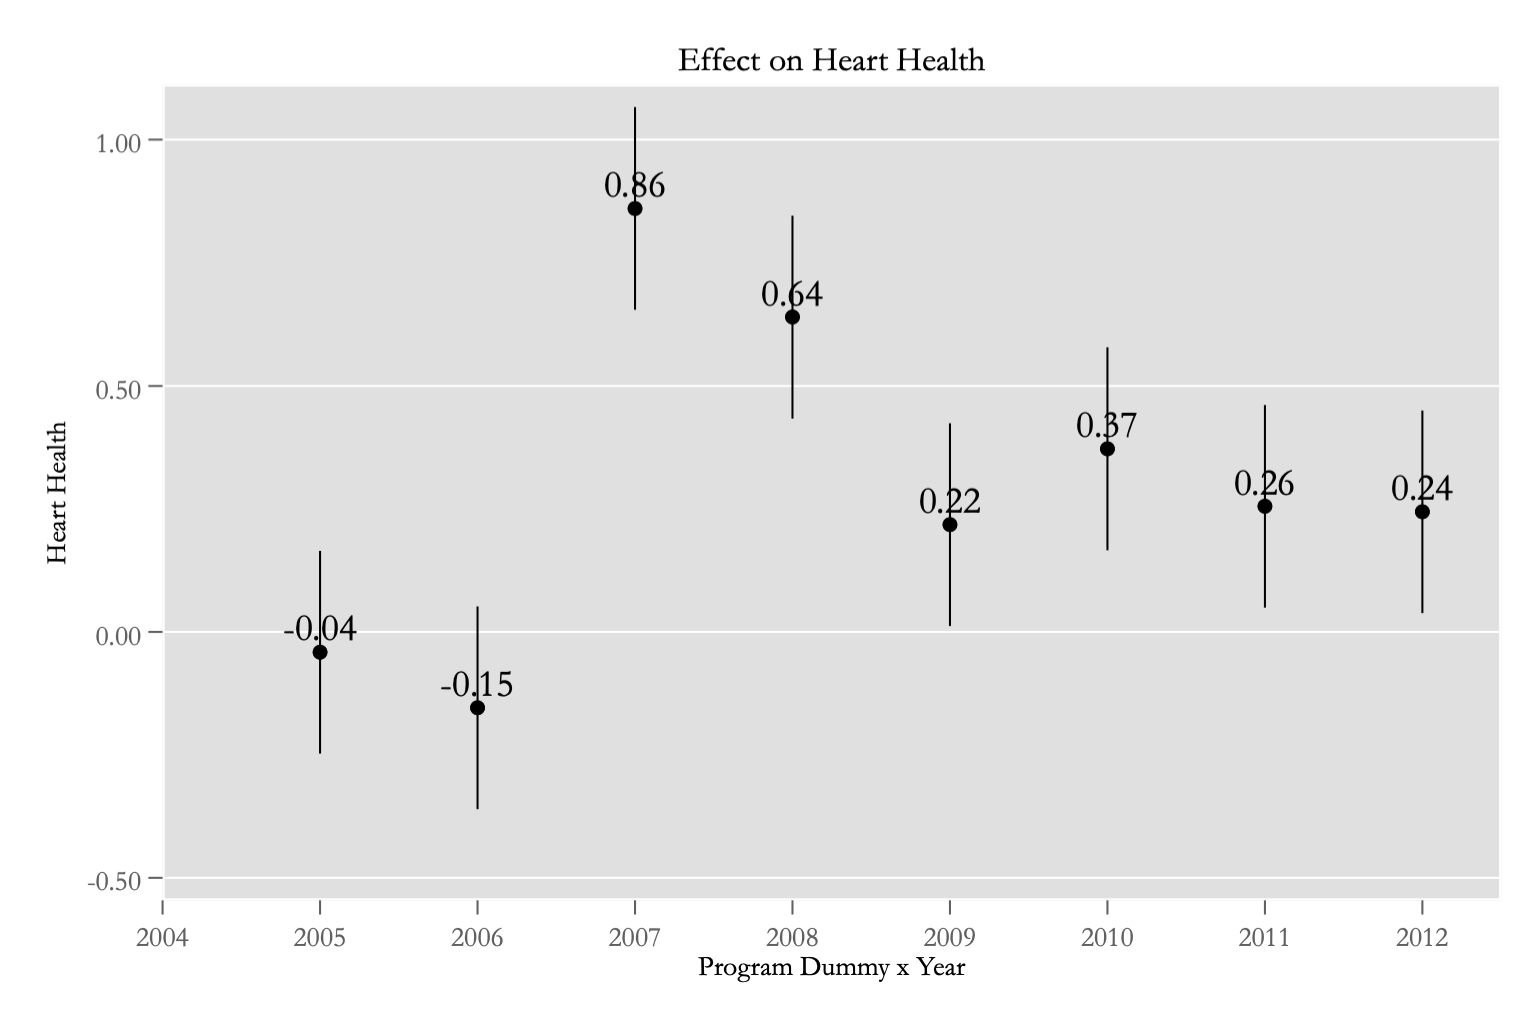
\includegraphics[width=.95\textwidth]{fig_year_heart.png}
 \caption{Causal Effect of Program on Heart Health by Year}
  \label{fig:SC}
 \end{figure}
 
Figure 1 shows a large immediate effect of treatment in 2007. Although this falls a bit in 2008, it is still clear how there exists an effect of treatment. In the years following treatment, treatment has less of an effect on outcome than the years during treatment. However, a positive difference in difference in outcome for treated people implies a small but lasting effect of treatment. As explained earlier, heart has no explicit interpretation so determining economic significance is up to interpretation. Visually seeing the effect of treatment throughout the years, I determine that the effect of treatment during the years of treatment is economically significant, but not economically significant in the years after treatment ended.
 

\begin{figure}[H]
\centering
 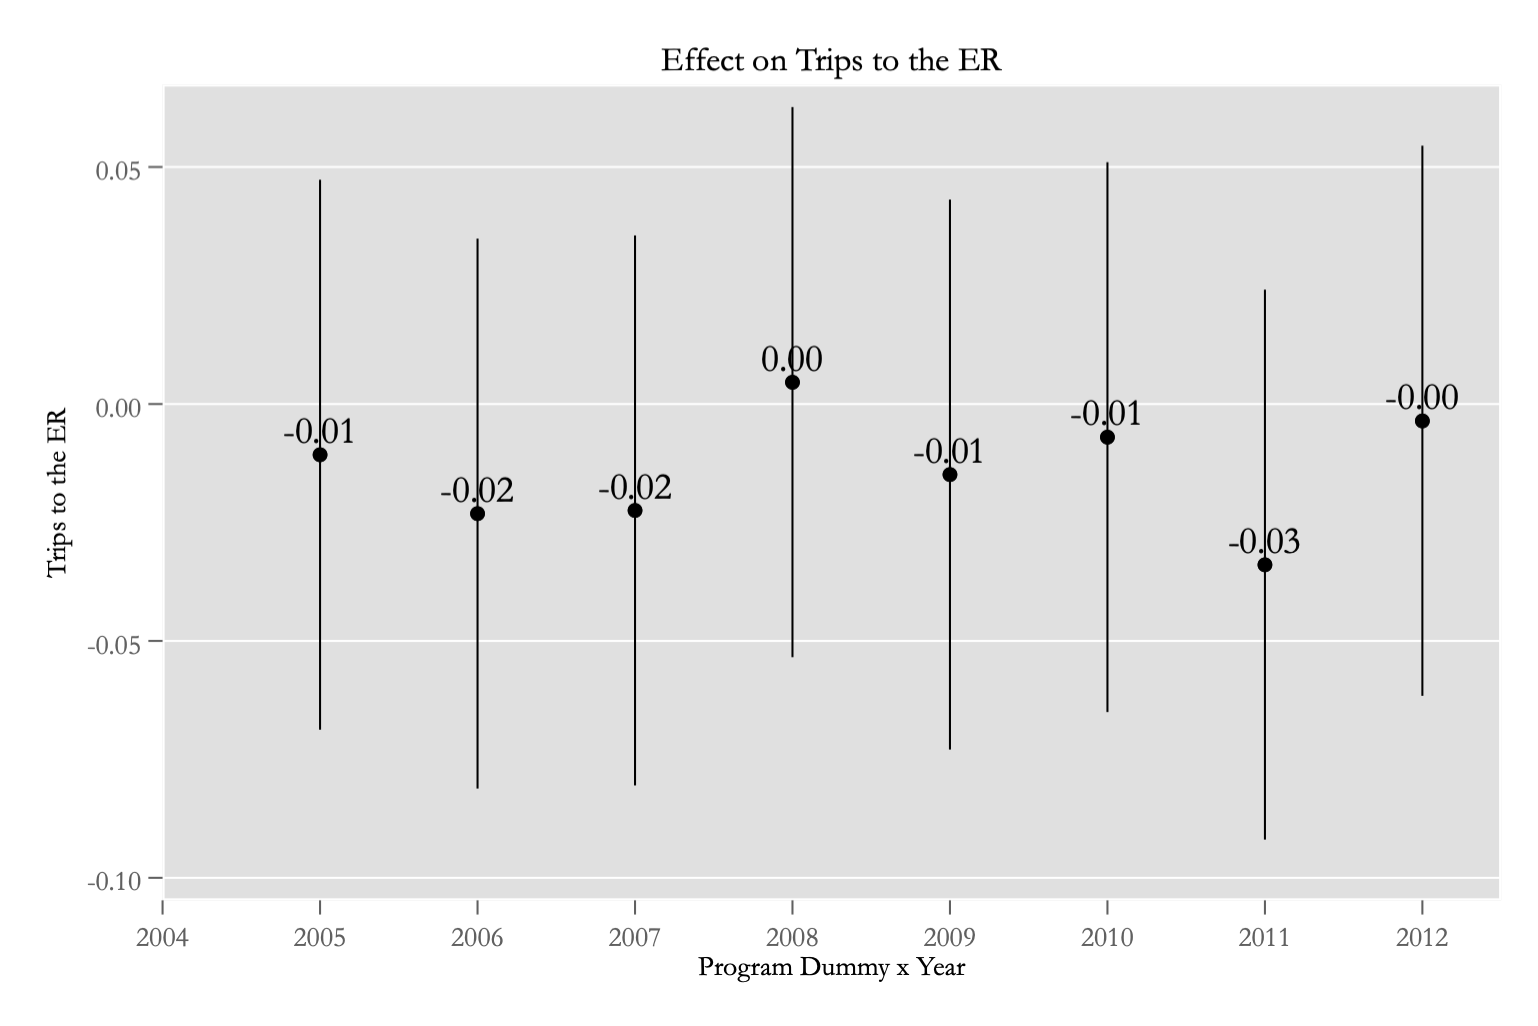
\includegraphics[width=.95\textwidth]{fig_year_er.png}
 \caption{Causal Effect of Program on Trips to the ER by Year}
  \label{fig:SC}
 \end{figure}
 
Figure 2 confirms that the effect of treatment on trips to the ER is economically insignificant. In 2007, the year that treatment starts, we see the effect of treatment is the same as it was in 2006, before treatment even started. In 2008, the number of trips to the ER actually increased; this makes little intuitive sense because one would expect a nutrition program to reduce the number of trips to the ER. There is no clear trend in the effect of treatment on outcome after treatment ends. Each year’s treatment effect is very close to zero; this provides strong support for my prior analysis that the treatment effect on trips to the ER is economically insignificant.


\begin{figure}[H]
\centering
 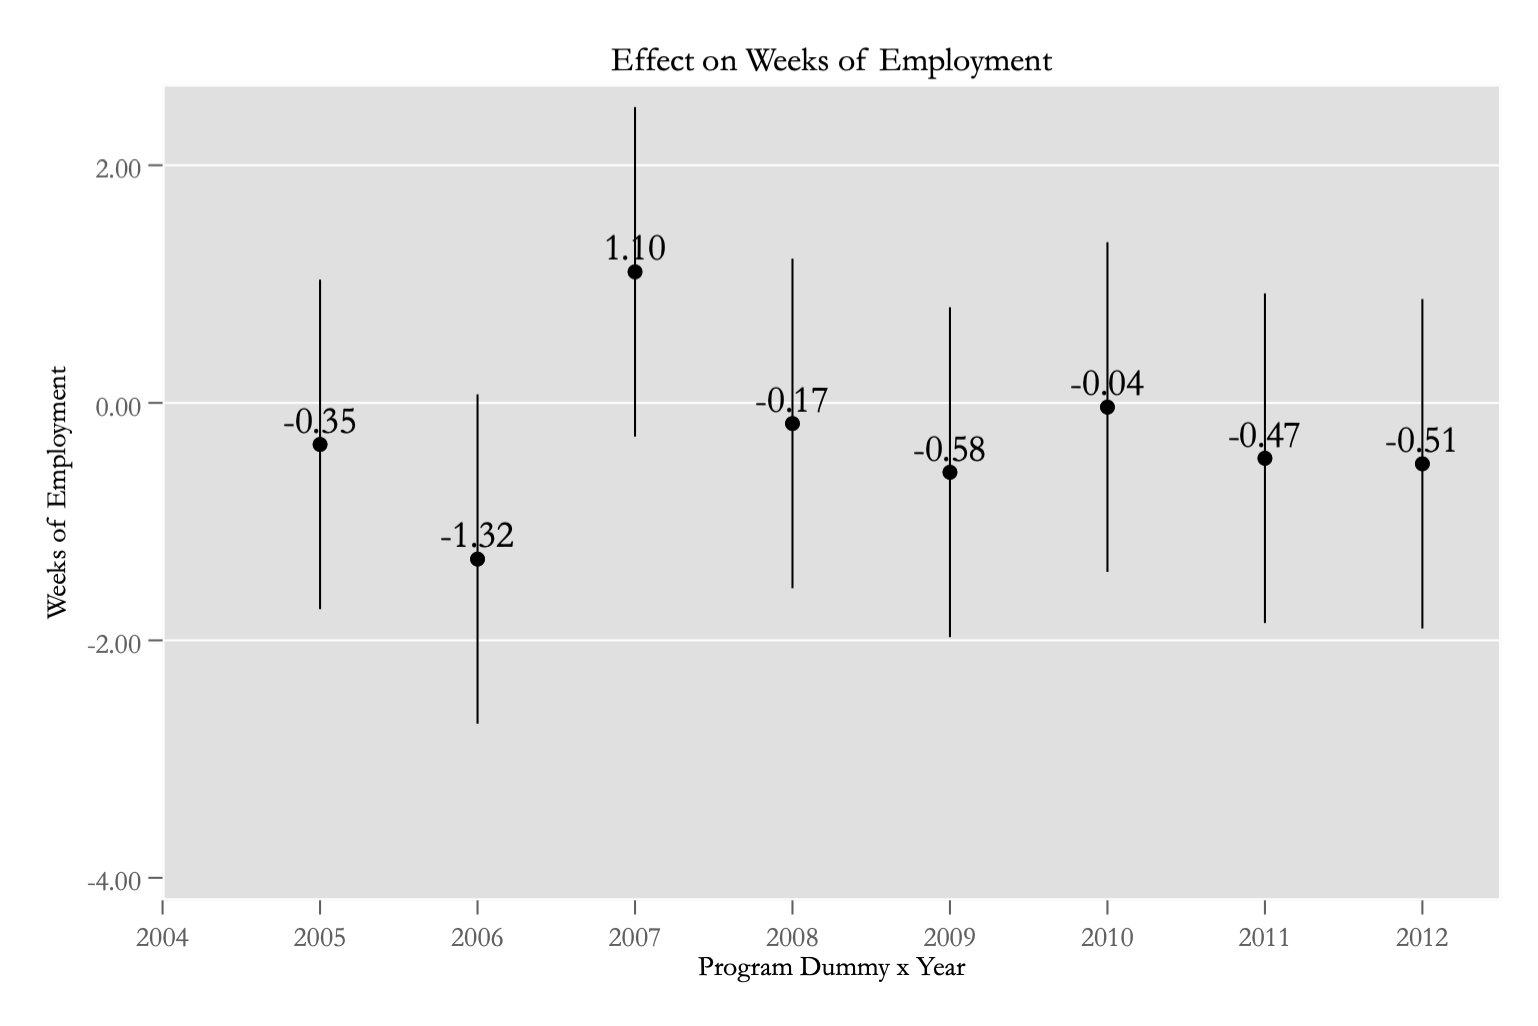
\includegraphics[width=.95\textwidth]{fig_year_employ.png}
 \caption{Causal Effect of Program on Weeks Employed by Year}
  \label{fig:SC}
 \end{figure}
 
In Figure 3, we see a jump in weeks of employment in 2007; this indicates some immediate effect of treatment. However, this effect is only 1.10; this is economically insignificant. In the second year of treatment, the outcome falls below zero. In the years after treatment ends, the effect of treatment is near zero and follows no particular trend; the effect of treatment on employment is economically insignificant.

%%##########################################################################

\section{Testing}

\subsection{Testing Hypotheses about a Single Parameter: t-test}

For each of the regressions specified in Equations 1 through 6, I conducted t-tests to determine the p-values of the estimated coefficients. For each of the regressions, I found p-values for the estimated coefficients on "Program dummy", "During treatment", "After treatment", "Program dummy*During treat", and "Program dummy*After treat". Respectively, these coefficients specified in Equations 1 to 6 are $\theta_1$, $\delta_2$, $\delta_3$, $\theta_2$, and $\theta_3$. These coefficients are unknown features of the population and we will never know them with certainty.  However, we can test hypotheses about the value of these coefficients using their estimated values and statistical inference. Thus, I tested the following:


\begin{equation}
\textbf{The null hypothesis $H_0: \theta_1 = 0$ against the alternative $H_1: \theta_1 \ne 0$}
\end{equation}
\begin{equation}
\textbf{The null hypothesis $H_0: \delta_2 = 0$ against the alternative $H_1: \delta_2 \ne 0$}
\end{equation}
\begin{equation}
\textbf{The null hypothesis $H_0: \delta_3 = 0$ against the alternative $H_1: \delta_3 \ne 0$}
\end{equation}
\begin{equation}
\textbf{The null hypothesis $H_0: \theta_2 = 0$ against the alternative $H_1: \theta_2 \ne 0$}
\end{equation}
\begin{equation}
\textbf{The null hypothesis $H_0: \theta_3 = 0$ against the alternative $H_1: \theta_3 \ne 0$}
\end{equation}

For an arbitrary coefficient $\beta_j$, the t-statistic $\hat{t_j}$ is calculated from the estimated value of the coefficient and equals $\hat{\beta_j} / se(\hat{\beta_j})$. We are interested in the probability that you would find a magnitude of $|\hat{\beta_j}|$ or higher if $\beta_j$ is indeed equal to zero, or \(P(t_{k-n-1} \ge \hat{t_j})\); this is the p-value. For each of the regressions, I find the p-value for each coefficient of interest. These can be seen in Tables 3, 4, and 5, for each of the three different dependent variables. 
I am interested in whether I reject or fail to reject the null hypotheses above, and whether this result changes as I control for variables. A very low p-value means the estimate for the coefficient was so unlikely to happen were the null actually true that we can reject the null; doing so rejects the idea that the corresponding independent variable has no effect on y. Likewise, a very high p-value means the estimate for the coefficient was very likely to happen if the null was true. In this case, we fail to reject the null and thus fail to reject the idea that the corresponding independent variable doesn't matter for determining y.

The reason for conducting these hypothesis tests is to establish statistical significance and see how test results change when control variables are added to the specification. Statistical significance is important for determining how confident we are that the observed results are real and not an error caused by randomness. Testing hypotheses establishes how reliable the results are. I am primarily interested in testing hypotheses for $\theta_2$ and $\theta_3$ but testing the other coefficients can paint a fuller picture.
\\
\\
For dependent variable heart, $\hat{\theta_1}$ has a very low p-value of 0.0000 across all four regressions. The estimate $\hat{\theta_1}$ is statistically significant and we reject the null that $\theta_1 = 0$ at the 1$\%$ level for all regressions. When no controls are present, $\hat{\delta_2}$ is statistically significant at the 5$\%$ level. However, adding age controls significantly raises the p-value such that $\hat{\delta_2}$ is statistically insignificant at the 10$\%$ level. This indicates that age had some explanatory power over the difference in outcome from the first period for untreated people in the second period. However, adding controls for education and age make $\hat{\delta_2}$ statistically significant at the 10$\%$ level, which just indicates some explanatory power of these two controls. With no controls, $\hat{\delta_3}$ was statistically insignificant at the 10$\%$ level. Adding age controls increase the p-value significantly; again, this means that controlling for age explained for some of the difference in outcome from the first period for untreated people in the third period. Adding education controls and county controls slightly decreased the p-value, again indicating these controls have some explanatory power. $\hat{\theta_2}$ and $\hat{\theta_3}$ both have very low p-values of 0.0000 across all four regressions. Thus, $\hat{\theta_2}$ and $\hat{\theta_3}$ are both statistically significant at the 1$\%$ level and we reject the nulls $\theta_2 = 0$ and $\theta_3 = 0$. This means we are confident at a very high level that the actual effect of treatment on heart health in periods 2 and 3 is not zero. 
\\
\\
For dependent variable er, $\hat{\theta_1}$ is the only estimate that is statistically significant at the 1$\%$ level. This means that we reject the null that the pre-existing difference captured in $\hat{\theta_1}$ is zero. However, all other estimates are statistically insignificant. The estimate $\hat{\delta_2}$ has a very high p-value of 0.96 when there are no controls. We fail to reject the null that $\delta_2 = 0$ at the 10$\%$ level. This makes since because the value of $\hat{\delta_2}$ is 0.0004, very close to zero. When adding controls, the value of $\hat{\delta_2}$ becomes even closer to zero. Correspondingly, the p-value is higher the closer $\hat{\delta_2}$ is to zero. Essentially, it becomes less likely that $\delta_2$ is not zero. For such a large sample size, this makes sense because the larger the sample size, the better the estimates. Similarly, $\hat{\delta_3}$ has a p-value of 0.69 when no controls are added, meaning we fail to reject the null that $\delta_3 = 0$. Again, we see the value of $\hat{\delta_3}$ is very close to zero, at -0.0043. Adding controls makes the estimate farther from zero, so the p-values for $\hat{\delta_3}$ decrease slightly. The same analysis is applied to the p-values for $\hat{\theta_2}$ and $\hat{\theta_3}$, whose estimates are also very close to zero. Adding controls makes $\hat{\theta_2}$ closer to zero so its p-values increase. Adding controls makes $\hat{\theta_3}$ farther from zero so its p-values decrease. The closer to zero the estimates are, the less likely we reject the null. These results show that we fail to reject that treatment has any effect on trips to the ER.
\\
\\
For dependent variable employ,  $\hat{\theta_1}$ has a very low p-value of 0.0000 across all four regressions. The estimate $\hat{\theta_1}$ is statistically significant and we reject the null that preexisting difference is zero at the 1$\%$ level for all regressions. In the regression without controls, $\hat{\delta_2}$ is statistically significant at the 5$\%$ level. However, adding controls increases the p-value enough that $\hat{\delta_2}$ is statistically insignificant at the 10$\%$ level and we fail to reject the null. This indicates that the control variables have explanatory power on the outcome. This is intuitive; a person’s age and level of education would have some effect on their number of weeks of education. When there are no controls, $\hat{\delta_3}$ and $\hat{\theta_2}$ are statistically insignificant at the 10$\%$ level and we fail to reject the null. $\hat{\delta_3}$ and $\hat{\theta_2}$ are both still statistically insignificant with even higher p-values when controls are added. Again, this indicates that the control variables have some explanatory power on the outcome. $\hat{\theta_3}$ is statistically significant at the 5$\%$ level for all four regressions. Thus, we fail to reject that $\theta_3 = 0$ at the 5$\%$ level. The p-value slightly increases when controls are added, again indicating the control variables have some explanatory power on the outcome. Thus we reject that the effect of treatment after treatment ended is zero. 

\subsection{Testing Multiple Linear Restrictions: F-test}

In order to see whether of a group of variables has no effect on the dependent variable, I test multiple restrictions in a joint hypothesis test. This test is to see whether the control variables age, educ, and county have no effect on the dependent variables, particularly to see whether all three jointly have no effect. This will tell me whether the regressions specified in Equations 4, 5, 6 are useful in analyzing the data. The coefficient on age is $\beta_1$, the coefficient on educ is $\beta_2$, and the coefficient on county is $\beta_3$. Thus, for the regressions specified in Equations 4, 5, and 6, I test the following hypotheses:

\begin{equation}
\textbf{The null $H_0: \beta_1 = 0$ against the alternative \(H_1: H_0\:is \:not\: true\)}
\end{equation}
\begin{equation}
\textbf{The null $H_0: \beta_1 = 0, \beta_2 = 0$ against the alternative \(H_1: H_0\:is \:not\: true\)}
\end{equation}
\begin{equation}
\textbf{The null $H_0: \beta_1 = 0, \beta_2 = 0, \beta_3 = 0$ against the alternative \(H_1: H_0\:is \:not\: true\)}
\end{equation}

The purpose of this test is the compare the predictive ability of the full specification with controls and the restricted model without controls specified in Equations 1 to 3. 

For this test we use the F-statistic $\hat{F}$, which can be calculated from $SSR_{res}$, the sum of squared residuals for the restricted model (no controls), and $SSR_{full}$ for the unrestricted model (with controls). The less the restricted model explains, the larger $\hat{F}$ becomes. 

The probability that we would see the difference $SSR_{res} - SSR_{full}$ as this value or larger, given the null is true, is the p-value of the F-test of this restriction. The p-value is interpreted the same way as for the t-test. A very low p-value means the $\hat{F}$ is very large and we can reject the null. This means that there is less explanatory power when excluding the controls; the controls are jointly statistically significant. We fail to reject the null for a very high p-value, meaning the controls are jointly insignificant and can justifiably be dropped from the model.

Although the F-test is generally used for testing the exclusion of multiple variables, I also tested the exclusion for the single control variable age to maintain consistency. The F-stat for excluding a single variable is equal to the t-stat squared. Both approaches lead to the same outcome because the alternative is two-sided.
\\
\\
For dependent variable $heart$, testing these three hypotheses yielded the following F-stat and p-value:
\begin{itemize}
    \item (12) F( 17, 58859) = 1.32, Prob > F = 0.1660
    \item (13) F( 21, 58855) = 167.79, Prob > F = 0.0000
    \item (14) F( 70, 58806) = 51.02, Prob > F = 0.0000
\end{itemize}
This first result tells me that the estimate $\hat{\beta_1}$ is statistically insignificant at the 10$\%$ level, meaning we fail to reject that adding controls for age adds no explanatory power at the 10$\%$ level. However, because the p-value is not too high, $\hat{\beta_1}$ is statistically significant at the 20$\%$ level. This is a very high significance level, so we reject the null that age controls have zero effect on outcome with low confidence. 

In the second result, we see that adding controls for education yields a very small p-value of 0.000. The estimates $\hat{\beta_1}$ and $\hat{\beta_2}$ are jointly statistically significant and we reject the null at the 1$\%$ level. Because we know that age controls are not statistically significant at a low significance level, this large drop in the p-value indicates that education controls adds explanatory power, and that $\hat{\beta_2}$ is likely statistically significant at a level lower than 16.6$\%$ level.

Unsurprisingly, in the third result, we see that adding controls for county yields the very small p-value of 0.0000 as well; The estimates $\hat{\beta_1}$, $\hat{\beta_2}$, and $\hat{\beta_3}$ are jointly significant at the 1$\%$ level. This is unsurprising because we already know that $\hat{\beta_1}$ and $\hat{\beta_2}$ are jointly significant with high confidence.

Because all three controls jointly add explanatory power to the baseline specification, I include all of them in the model.\\
\\
For dependent variable $er$, testing these three hypotheses yielded the following F-stat and p-value:
\begin{itemize}
    \item (12) F( 17, 60349) = 1.44, Prob > F = 0.1070
    \item (13) F( 21, 60345) = 1.30, Prob > F = 0.1634
    \item (14) F( 70, 60296) = 1.22, Prob > F = 0.1049
\end{itemize}

This first result tells me that the estimate $\hat{\beta_1}$ is statistically insignificant at the 10$\%$ level, meaning we fail to reject that adding controls for age adds no explanatory power at the 10$\%$ level. However, because the p-value is not too high, $\hat{\beta_1}$ is statistically significant at the 20$\%$ level. This is a very high significance level, so we reject the null that age controls have zero effect on outcome with low confidence. 

In the second result, we see that adding controls for education yields a larger p-value. The estimates $\hat{\beta_1}$ and $\hat{\beta_2}$ are jointly insignificant and we fail to reject the null at the 10$\%$ level.
This tells me that adding education controls do not add explanatory power; education is likely unrelated to the dependent variable er. 

In the third result, we see that adding controls for county yields a smaller p-value. Although we still fail to reject the null at the 10$\%$ level, the estimates $\hat{\beta_1}$, $\hat{\beta_2}$, and $\hat{\beta_3}$ are jointly significant at the 11$\%$ level. Having all three controls adds more explanatory power than just controlling for age, or just controlling for age and education.
\\
\\
For dependent variable $employ$, testing these three hypotheses yielded the following F-stat and p-value:
\begin{itemize}
    \item (12) F( 17, 59752) = 1.74, Prob > F = 0.0299
    \item (13) F( 21, 59748) = 4.47, Prob > F = 0.0000
    \item (14) F( 70, 59699) = 1.92, Prob > F = 0.0000
\end{itemize}
The first result shows that the estimate $\hat{\beta_1}$ is statistically significant at the 2.5$\%$ level, meaning we fail to reject that adding controls for age adds no explanatory power at the 2.5$\%$ level.

The second result shows that controlling for education as well adds even more explanatory power; the low p-value means that the estimates $\hat{\beta_1}$ and $\hat{\beta_2}$ are jointly significant at the 1$\%$ level and we reject the null with high confidence. 

The third result shows that the estimates $\hat{\beta_1}$, $\hat{\beta_2}$, and $\hat{\beta_3}$ are jointly significant at the 1$\%$ level. This is unsurprising because we know that $\hat{\beta_1}$ and $\hat{\beta_2}$ are jointly significant at a very low significance level.

\section{Threats}

\begin{itemize}
\item \textbf{Missing Data}
\end{itemize}
\\
As we can see from Table 1, the initial data had missing data values for educ, age, employ, and heart. Although the missing values for age and education could be replaced with the correct values, there is no way to fill in the missing heart and employ values. This becomes problematic when the missing data is a nonrandom sample. We are unable to determine if the data is missing at random so this threatens the ability to find the causal effect of treatment. 

The missing values for heart and employ become problematic when the missing data is correlated with the dependent variable, which implies it is related to $u$. For example, people with low employment in a particular year might be more likely to not report their weeks of employment on a survey. Or, individuals whose heart health was significantly lower in a particular year might be less willing to report their heart health for the year. These are both valid possibilities that present bias if true.

Replacing heart values of 9999 as missing could also introduce bias if these values are related to the dependent variable. I assume that the value 9999 is used to code for missing, but it is possible that this value is systematically related to the heart value. For example, they could represent heart values greater than a certain threshold. The maximum heart value seen in Table 2 is just over 21; perhaps the value 9999 represents heart values larger than 22. Using a sample of people with missing data for heart health above 22 results in biased and inconsistent estimators. 

\begin{itemize}
\item \textbf{Program Selection}
\end{itemize}
\\
There is no information on how the people were chosen to be in the program. This present a threat because we cannot assume that selection was random. In order to be unbiased, the treated group cannot have a different time trend than the untreated group. A different time trend means that $E[u_{ij}|Program_i x Period_j] \ne 0$ and the estimates of the effect of treatment $\theta_2$ and $\theta_3$ are biased. 

We can see whether the treated group was following a different time trend prior to treatment in Figures 1, 2, and 3. In the years before treatment, 2005 and 2006, treated people should not have a difference in outcome and $\theta_{2005}$ and $\theta_{2006}$ should be close to zero. 

In Figure 1, we see that the difference in outcome for treated people decreased from 2005 to 2006 and was -0.15 in 2006. For the small range of values for heart health, this value is not as close to zero as it should be. In Figure 2, the difference in outcome also decreases from 2005 to 2006. The difference in outcome prior to treatment is very close to the difference in outcome during and after treatment. Finally, in Figure 3, the difference in outcome decreases prior to treatment. The difference in outcome in 2006 is larger than any difference in outcome following 2007.

All three figures show that the difference in outcome prior to treatment is not zero. This violates the parallel trend requirement. Treated people are seeing a change in their outcome that is different from untreated people even before treatment starts, creating bias in our estimates of the effect of treatment. Thus we can't determine a causal effect.

\begin{itemize}
\item \textbf{Unobservables}
\end{itemize}
\\
Although I add controls for age, education, and county, it is very likely that there exists other unobserved variables that effect the outcome. For example, income is an unobserved variable that could impact the outcome significantly. Healthy food is generally more expensive than junk food and gym memberships can be expensive. A person's economic status could have a large impact on their ability to eat healthy and exercise. If the effect of unobservables like income on outcome are not zero and we don't control for them, our estimates are biased.

Thus, I control for all observable variables age, education, and county to alleviate concerns that estimates are biased without them. Using F-tests, I determined that these controls were jointly significant and I am thus justified in keeping them in my model. 

\begin{itemize}
\item \textbf{Statistical Insignificance}
\end{itemize}
\\
Statistical insignificance inhibits our ability to determine a causal effect. As I mention in testing, statistical insignificance makes it difficult to determine economic significance because we cannot reject that the estimate of a coefficient is zero. We therefore cannot determine causality for estimates with high p-values.

I test hypotheses and find p-values because determining statistical significance alleviates concerns about making a causal interpretation.

\begin{itemize}
\item \textbf{Interpretation of $heart$}
\end{itemize}
\\
It is difficult to determine a causal effect of treatment on heart health when there is no explicit interpretation of heart. Pre-existing heart issues may not be fixed just from exercise and nutrition. Heart muscle is also one of the least renewable tissues in the body, so someone with permanent heart damage may not be able to improve their $heart$ value even if they improve their nutrition and exercise. The dependent variable $heart$ is very arbitrary and thus makes it difficult to determine a causal effect of treatment. 
\\
\vspace{2mm}
\\
Although I add controls and test hypothesis about the estimates, the analysis of results and threats mentioned make me reluctant to establish a causal effect of treatment on heart health, trips to the ER, and weeks of employment. 


\vspace{2mm}

\end{document}


